\documentclass{article}
\usepackage{amsmath,amssymb}
\usepackage{tikz}
\usetikzlibrary{arrows.meta,positioning,calc,shapes.geometric}
\pagestyle{empty}
\begin{document}
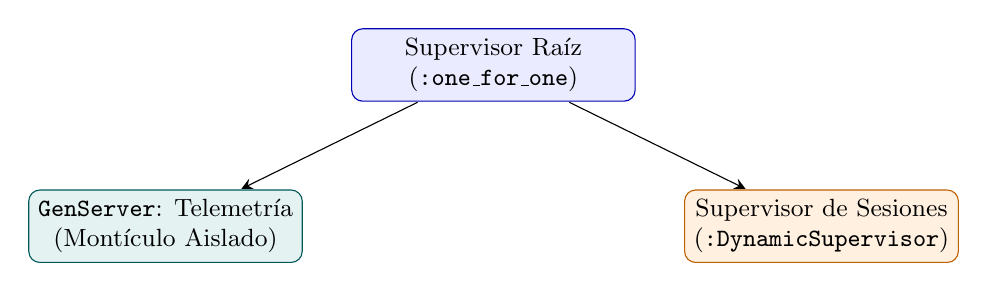
\begin{tikzpicture}
\tikzset{node distance=1.4cm, >=stealth, thick, font=\small}
\node[draw=blue!70!black, fill=blue!8, rounded corners, minimum width=3.6cm, minimum height=0.9cm, align=center] (root) {Supervisor Raíz\\(\texttt{:one\_for\_one})};
\node[draw=teal!70!black, fill=teal!10, rounded corners, minimum width=3.2cm, minimum height=0.9cm, align=center, below left=1.1cm and 0.6cm of root] (w1) {\texttt{GenServer}: Telemetría\\(Montículo Aislado)};
\node[draw=orange!75!black, fill=orange!12, rounded corners, minimum width=3.4cm, minimum height=0.9cm, align=center, below right=1.1cm and 0.6cm of root] (sub) {Supervisor de Sesiones\\(\texttt{:DynamicSupervisor})};
\draw[->] (root) -- (w1);
\draw[->] (root) -- (sub);
\end{tikzpicture}
\end{document}
